\section{Structure}\label{sc:structure}
% Intro intro
Based on the analysis in the former sections, the structure of the classes in the problem domain has been visualised in a class diagram (see \autoref{fig:FirstPDClassDiagram}).

\begin{figure}[H]
    \centering
    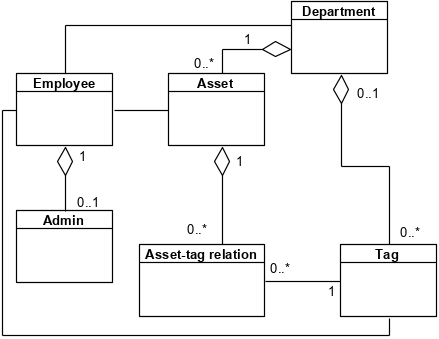
\includegraphics[width=0.8\textwidth]{figures/ClassDiagrams/Class_activity_class_diagram.png}
    \caption{Class diagram of the classes in the problem domain.}
    \label{fig:FirstPDClassDiagram}
\end{figure}

As described in \autoref{sc:classes}, there are six different relevant classes in the problem domain. These classes are: \textit{Employee}, \textit{Admin}, \textit{Department}, \textit{Asset}, \textit{Tag}, and \textit{Asset-tag relation}. The relations between these have been explained below.
\par

The \textit{Employee} class is an aggregation of the \textit{Admin} class. The structure created by this connection is a role pattern with only one role. The pattern makes it possible for an employee to possess the role of \textit{Admin} dynamically.
\par

The \textit{Asset} aggregates a number of \textit{Asset-tag relation}s. On top of this, every asset belongs to one department.
\par

The \textit{Employee} class has a association to the \textit{Asset}, \textit{Department}, and \textit{Tag} classes, as they can see the information on an asset and search for through them based on tags and/or departments. The \textit{Admin} class is a role of the \textit{Employee} class. This means that the functionality kept in the \textit{Admin} class will be available to the employees who have the role of admin.
\par

The \textit{Asset-tag relation} class is created to handle the relation between the \textit{Asset} and \textit{Tag} classes. The \textit{Asset} class aggregates it, as an asset the tags exists only as an addition to the assets. It has been added, as multiple assets can be tagged with the same tag and an asset can have multiple tags. The association to the \textit{Tag} class originates from the relation pattern. An instance of the \textit{Asset-tag relation} class always connects one asset and one tag, but both the \textit{Tag} and \textit{Asset} classes can be part of mulitple asset-tag relations.
\par

With the classes of the problem domain and their interconnecting relations described, the behaviour of the classes can be examined.